%!TEX root = vorlage.tex

\subsection{The data}

The experiments were done on the \textit{Instrument segmentation and tracking}
dataset of the Endoscopic Vision Challenge
\enquote{EndoVis}\footnote{\href{http://endovis.grand-challenge.org/}{http://endovis.grand-challenge.org}}.
It contains photos of minimal-invasive operations. The dataset already contains
a training-test-split. The training data consists of four operations. Each
operation has 40~RGB~images in a resolution of $\SI{640}{\pixel} \times
\SI{480}{\pixel}$. The test set has 10~more images of those 4~operations as
well as 50~images for 2~more operations. This means, in total the training data
consist of $4 \cdot 40 = 160$ photos and the testing contains $4 \cdot 10 + 2
\cdot 50 = 140$ photos. As each pixel has to be classified as \textit{medical
instrument} or \textit{background}, there are
$140 \cdot 640 \cdot 480 = \num{43008000}$ classifications to be done for
testing.

The training data consist of $\SI{90.5}{\percent}$ background
($\SI{90.8}{\percent}$ in the testing data); the remaining pixels are medical
instruments. This means an accuracy of $\SI{90.8}{\percent}$ can be reached
without looking at the test image.

Analyzing the data, one can also see that some positions in the image are more
likely than others to contain a medical instrument. This is visualized
in~\cref{fig:medical-instrument-positions}.

\begin{figure}[ht]
    \centering
    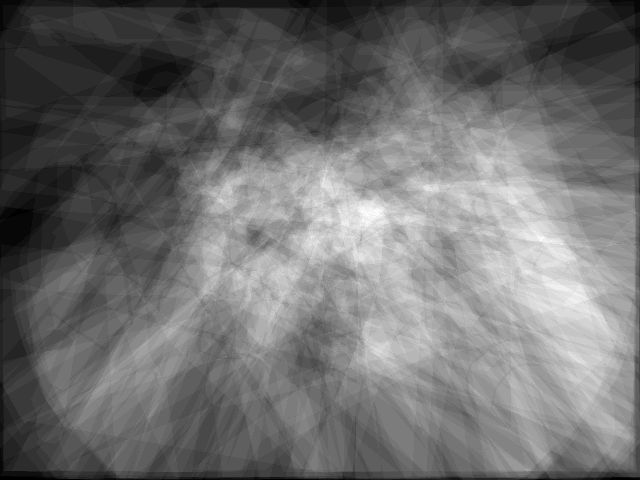
\includegraphics[width=\linewidth]{images/instrument-positions.png}
    \caption{Position of medical instruments in the training data.
             The brighter the color, the more often was a medical instrument
             at this position. One can clearly see that the borders contain
             medical instruments less often. Also, in the center they are much
             more often.}
    \label{fig:medical-instrument-positions}
\end{figure}
